\chapter{Problembeskrivelsen}

I dette afsnit vil den endelige problemformulering blive beskrevet, samt kravene til den endelige løsning. Til sidst afgrænses der i forhold til gruppens evner og de krav der er blevet opstillet. 

\section{Problemafgrænsning}
Ud fra denne analyse, kan der konkluderes, at VisitAalborg og turisterne er ressourcepersoner, hvoraf turisterne har større indflydelse på programmet, da der er de endelige brugere. VisitAalborg kan bruges som guider til, hvad der kan være af indhold i programmet, men der skal stadig tages højde for, at det er i deres interesse, at få deres arbjedspartnere med ind i programmet, selvom det ikke i alle tilfælde er til turistens interesse.
Ved spørgeskemaet blev der uddraget, at turister allerede har løsninger fra punkt til punkt, hvor der i eksisterende løsninger blev påpeget, at der også findes løsninger for fler-punktsruter. TripAdvisor viste, at der også er programmer, som tager højde for brugerens interesse, men alt taget i betragtning, er der ikke en løsning der kombinerer alle disse funktioner, som der belyses i gruppens spørgeskema og interview, til at være i brugerens bedste interesse: En simpel løsning, der inddrager brugerens interesse, og foreslår yderligere punkter til en mere interessant rute. Dette kunne endda optimiseres ved en offline-funktion, som TripAdvisor også gør brug af ved et offline kort.

\section{Problemformuleringen}
Hvordan udvikles der en softwareløsning, der hjælper turisten med at finde rundt i en storby, på en interessant rute mellem turistens egne valgte attraktioner?

\section{Kravspecifikationer}
I dette afsnit vil gruppen kigge og vurdere, hvilke krav der skal indegå i en løsning. Heri vil der både blive opstillet krav til en optimal løsning og til en afgrænset løsning, som gruppen mener at være realistisk, at kunne lave.

\subsection{Optimale løsningsforslag}
For at kunne udvilke en softwareløsning, der besvarer gruppens problemformulering, er det vigtigt at definere nogle krav til programmet. Til en optimal løsning, har gruppen vurderet, at der skal være følgende krav:
\begin{itemize}
	\item Programmet skal udvikles som en applikation til moderne smartphones, inklusiv iOS, Android og Windows Phone. 
	\item Programmet skal vise et kort med ruten, og på kortet vise attraktioner der er tæt på. 
	\item Programmet skal kunne beregne den korteste rute mellem en række punkter.
	\item Det skal være muligt at få programmet til at vise rutevejledningen, på samme måde som normale GPS-enheder. 
	\item Programmet skal give mulighed for at bedømme attraktioner, og derved tildele dem en rating. Dette skal bruges til at rangere attraktionerne, for at hjælpe turisterne med at vælge den mest interessante rute. 
	\item Det skal være i stand til at give forslag til en anden rute, der inkludere attraktioner der ligger tæt på ruten.
	\item Der skal være mulighed for at downloade en offline version af den rute der er valgt, inklusiv kortet for det omkringliggende område. Dette er for at hjælpe dem der ikke har billig data hvor de bruger programmet.
\end{itemize}
Til disse krav har gruppen konstrueret nogle skitser af den optimale løsning, for at give et billede af hvordan det eventuelt kunne se ud. \newline

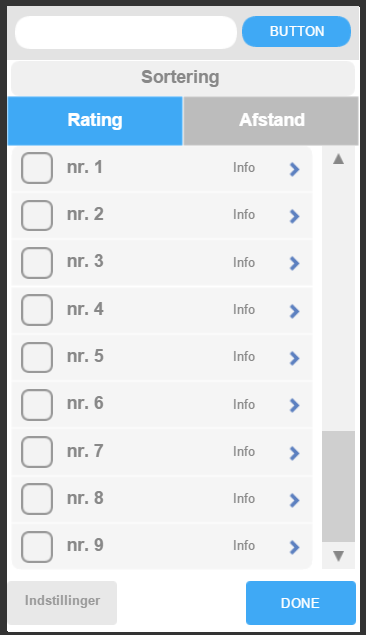
\includegraphics[scale=0.35]{start1} \newline
Denne skitse viser den overordnede brugergrænseflade. Gruppen ønsker, at programmet skulle fungere på den måde, at der findes to valg muligheder, forholdsvis rating og afstand, hvoraf rating viser en række attraktioner med en værdi, baseret på hvad brugerne har valgt at rate den. Funktionen afstand, vil vise hvor stor en afstand der er fra det punkt hvor brugeren står, til en attraktion. De attraktioner, som brugeren ønsker at se, skal brugeren blot tjekke af, ved at klikke på attraktionerne (I dette tilfælde nr. 1, nr. 2 etc), og de vil derefter blive tilføjet til den nuværende rute. 


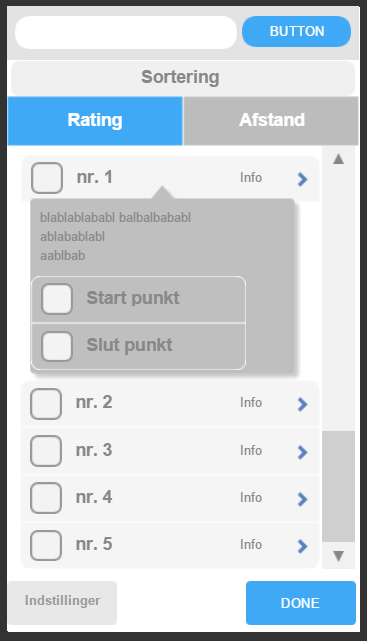
\includegraphics[scale=0.35]{start2} \newline
Denne skitse viser en udvidet brugergrænseflade, hvor brugeren har valgt at klikke på drop-down-menuen "info". Denne menu vil derefter give bruger nogle informationer omkring attraktionen. Den vil derudover have to yderligere muligheder, start- og slutpunkt. Disse funktioner kan brugeren fx anvende, hvis der er en ønsket slut/start-lokalisation, hvor programmet derefter skal beregne den ønskede rute ud fra.


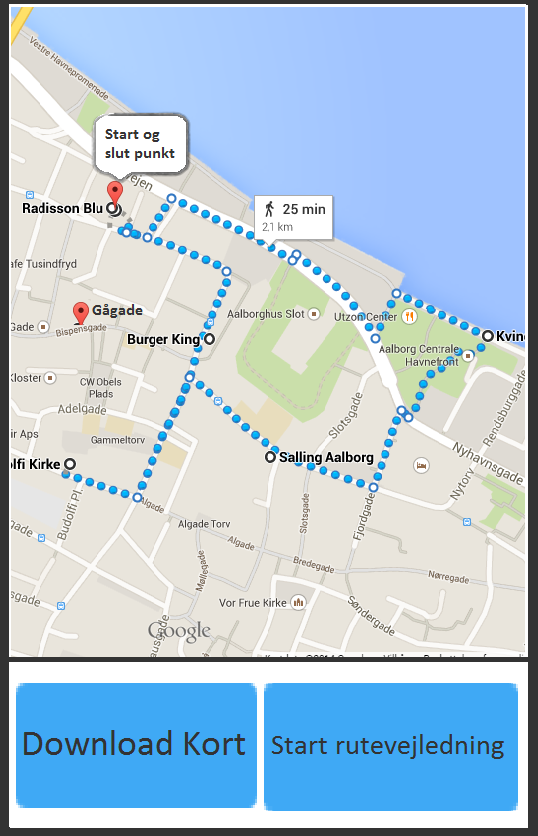
\includegraphics[scale=0.3]{rute1} \newline
Følgende skitse viser hvordan ruten fremvises, efter brugeren har valgt de attraktioner, som der ønskes at besøge. Ruten der vises, viser hvor lang hele ruten er, og hvor lang tid det tager at gå ruten. Herudover er der to knapper brugeren kan vælge at benytte sig af. Den ene knap er "download kort", som downloader kortet på mobilen, og derved gør det muligt at anvende programmet, uden at skulle bruge internet. Den anden knap "Start rutevejledning" viser vej og fortæller brugeren, hvornår han skal dreje etc. 


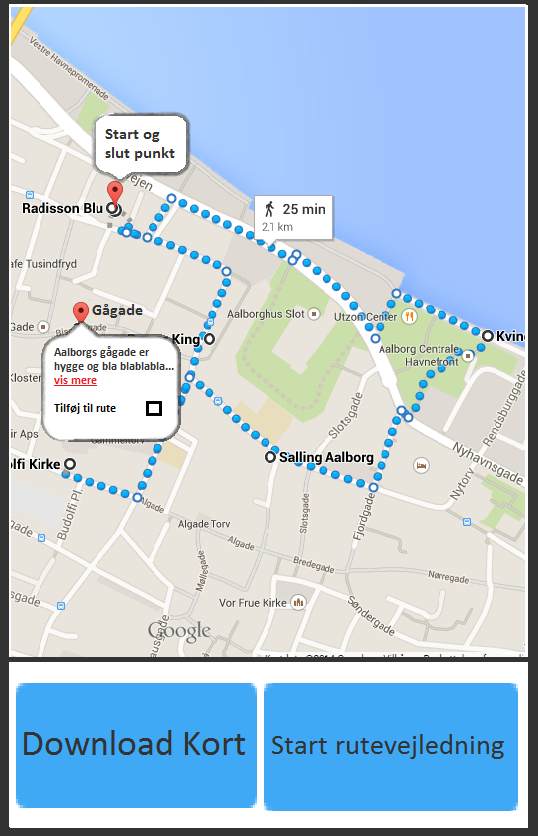
\includegraphics[scale=0.3]{rute2} \newline
Denne skitse er blot en udvidet version af den tidligere skitse. Forskellen på disse skitser er blot, at der i denne model, er vist hvordan der kan tilføjes flere punkter til den nuværende rute. Alle ikonerne på kortet, skal kunne klikkes på, hvor så der er mulighed for at tilføje disse punkter til ruten, hvis det ønskes, af brugeren. Herudover er der en "vis mere"-funktion, som vil vise informationer om attraktionen, brugeren har valgt, på samme måde som ved figur 2. 

\subsection{Gruppens løsningsforslag}
Gruppen har gennem spørgskema og interview, fået stillet en række krav til løsningen, af turister og VisitAalborg. 
Gennem spørgskemaet, blev det konkluderet, at det vigtigste for turister, er at de kan opleve byen på en interessant rute. 
Derudover har turistbureauet givet udtryk for, at løsningen gerne skal være så enkelt som muligt, altså meget få funktioner, så brugeren ikke bliver forvirret, da de mener, at det er i turistens bedste interesse. \newline
Der er blevet stillet krav fra universitets side, om at programmet skal være et lille specifikt program i C, af høj kvalitet. Dette stemmer godt overens, med de krav der er blevet stillet fra turistbureauets side.   \newline
Ud fra dette, har gruppen opsat nogle krav for gruppens løsningsforslag, og de er som følgende:
\begin{itemize}
	\item Programmet skal kunne beregne den korteste rute mellem en række punkter.
	\item Det skal være i stand til at give forslag til en anden rute, der inkludere attraktioner der ligger tæt på ruten.
 	\item Der skal som output, gives en liste over rutens destiationer, sorteret efter hvilken rækkefølge er hurtigst.
\end{itemize}

Da dette er et P1 projekt, og gruppen er begrænset af både tid og erfaring, har gruppen valgt at begrænse softwareløsningen, på følgende punkter: 
\begin{itemize}
	\item Rutevejledningen bliver i fugleflugtslinje.
	\item Brugeren kan kun vælge destinationer ud fra en række forudbestemte punkter.
	\item Tekstbaseret brugergrænseflade.
\end{itemize}

På baggrund af kravene og afgrænsningen, har gruppen tænkt sig at lave et program, som har nogle forudbestemte destinationer, der dækker over destinationerne i Aalborg, hvorefter brugeren vælger de destinationer han/hun ønsker at besøge. Programmet vil ud fra disse punkter, beregne den korteste rute, og undersøge om der er andre attraktioner, som ligger tæt på ruten, og spørge brugeren, om det kunne være interessant at besøge disse steder. Hvis ja, vil disse punkter også blive inkluderet. Resultatet bliver en liste over destinationerne, der står i rækkefølge, så turisten ved hvilken rækkefølge de skal besøge dem i, for at få den mest optimale rute.
